\chapter{Case Studies and Applications}

\section*{Scenario 1: Ideal Harvesting Time for Hilly Areas}

Farmers in hilly areas often struggle to decide the best time to harvest crops. Certain crops thrive only under specific environmental conditions—neither too hot nor too wet. With the help of climate data analysis, we aim to provide a data-driven recommendation.

\subsection*{Objective}
Identify the months in which both temperature and rainfall are within a moderate range, ideal for harvesting.

\subsection*{Step 1: Understanding the Data}
We use a dataset containing daily climate observations. The relevant variables for this case study include:
\begin{itemize}
  \item \textbf{Temp\_2m}: Daily average temperature (°C)
  \item \textbf{Precip}: Daily total precipitation (mm)
  \item \textbf{Month}: Month extracted from the date
\end{itemize}

\subsection*{Step 2: Define Moderate Conditions}
To define what constitutes a ``moderate'' range for temperature and rainfall, we calculate the 25th and 75th percentiles. This approach, known as the interquartile range (IQR), captures the central 50\% of the data, filtering out extreme values.

\textbf{R Code:}
\begin{verbatim}
temp_range <- climate_data %>%
  summarise(
    q25_temp = quantile(Temp_2m, 0.25, na.rm = TRUE),
    q75_temp = quantile(Temp_2m, 0.75, na.rm = TRUE)
  )

precip_range <- climate_data %>%
  summarise(
    q25_precip= quantile(Precip, 0.25, na.rm = TRUE),
    q75_precip = quantile(Precip, 0.75, na.rm = TRUE)
  )
\end{verbatim}

\textbf{Mathematically, the moderate ranges are defined as:}
\[
\text{Moderate Temperature Range} = \left[ Q^{\text{Temp}}_{25},\; Q^{\text{Temp}}_{75} \right]
\]

\[
\text{Moderate Rainfall Range} = \left[ Q^{\text{Precip}}_{25},\; Q^{\text{Precip}}_{75} \right]
\]

\begin{verbatim}
moderate_temp_range <- c(temp_range$q25_temp, temp_range$q75_temp)
moderate_rainfall_range<-c(precip_range$q25_precip, precip_range$q75_precip)

# Print moderate ranges
moderate_temp_range
moderate_rainfall_range
\end{verbatim}

\subsection*{Step 3: Analyze Monthly Averages}
With the moderate ranges established, we now compute the monthly averages of temperature and rainfall. We then identify months whose averages fall within both moderate ranges.

\textbf{R Code:}
\begin{verbatim}
monthly_summary <- climate_data %>%
  group_by(Month) %>%
  summarize(
    avg_temp = mean(Temp_2m, na.rm = FALSE),
    avg_precip = mean(Precip, na.rm = FALSE)
  )
suitable_months <- monthly_summary %>%
  dplyr::filter(
    avg_temp >= moderate_temp_range[1] & avg_temp <= moderate_temp_range[2],
    avg_precip >= moderate_rainfall_range[1] & 
avg_precip <= moderate_rainfall_range[2]
  )
print(suitable_months)
\end{verbatim}

\textbf{Based on this analysis, the following months are identified as having both moderate temperature and moderate rainfall:}

\begin{table}[h!]
\centering
\begin{tabular}{|c|c|c|}
\hline
\textbf{Month} & \textbf{Average Temperature (°C)} & \textbf{Average Precipitation (mm)} \\
\hline
Mar & 13.8 & 0.547 \\
Apr & 18.4 & 0.801 \\
Oct & 15.8 & 1.15 \\
Nov & 12.0 & 0.134 \\
\hline
\end{tabular}
\caption{Average temperature and precipitation values for selected months.}
\end{table}

These months are ideal for harvesting crops that are sensitive to extreme weather conditions.

\subsection*{Conclusion}
This case study demonstrates how statistical concepts—specifically percentiles and the interquartile range—can be applied to real-world agricultural planning. Using R, we processed climate data to guide harvesting decisions in hilly regions. This approach exemplifies how climate analytics can directly support informed, local decision-making.

\section*{Scenario 2: Disaster Preparedness — Identifying Flood-Prone Regions}

Flood preparedness is a crucial step in climate resilience, particularly in regions where seasonal rainfall patterns lead to recurring floods. By analyzing historical rainfall data, we can identify areas most at risk and proactively design early warning systems, resource allocation strategies, and infrastructure improvements.

\subsection*{Objective}
\begin{itemize}
    \item Identify the top 5 regions with the highest average rainfall.
    \item Recommend the months in which flood alerts should be heightened based on high monthly rainfall.
\end{itemize}

\subsection*{R Code for Analysis}
\textbf{Top 5 Rainfall-Prone Regions:}
\begin{verbatim}
# Aggregate rainfall by region
region_rainfall <- climate_data %>%
  group_by(District) %>%
  summarise(avg_rainfall = mean(Precip, na.rm = TRUE)) %>%
  arrange(desc(avg_rainfall))

# Show the top 5 regions with highest rainfall
top_regions <- head(region_rainfall, 5)
print(top_regions)
\end{verbatim}

\begin{table}[h!]
\centering
\begin{tabular}{|c|c|}
\hline
\textbf{District} & \textbf{Average Rainfall (mm)} \\
\hline
Ilam & 3.64 \\
Jhapa & 3.39 \\
Argakhanchi & 3.03 \\
Rupandehi & 3.03 \\
Palpa & 3.02 \\
\hline
\end{tabular}
\caption{Top 5 Rainfall-Prone Districts}
\end{table}

\subsection*{Monthly Rainfall in Top Regions}

To identify critical months for potential flood risks, we examined the monthly average rainfall in each of the top-ranking districts. This analysis highlights temporal patterns of precipitation, allowing for a clearer understanding of seasonal variability. Months with the highest recorded precipitation in each district should be prioritized in flood alert planning and early warning systems.


\textbf{R Code:}
\begin{verbatim}
monthly_rainfall <- climate_data %>%
  filter(District %in% top_regions$District) %>%
  group_by(District, Month) %>%
  summarize(Monthly_Rainfall = mean(Precip, na.rm = TRUE)) %>%
  arrange(District, desc(Monthly_Rainfall))

ggplot(monthly_rainfall, aes(
  x = District, y = Monthly_Rainfall, fill = Month)) +
  geom_bar(stat = "identity", position = "dodge") +
  scale_fill_brewer(palette = "Set3") +
  labs(
    title = "Monthly Rainfall Distribution in Top Regions",
    x = "District",
    y = "Average Monthly Rainfall (mm)",
    fill = "Month"
  ) +
  theme_minimal() +
  theme(
    axis.text.x = element_text(angle = 45, hjust = 1),
    legend.position = "right"
  )
\end{verbatim}

% Figure here-----------------------------
\begin{figure}[h]
\centering
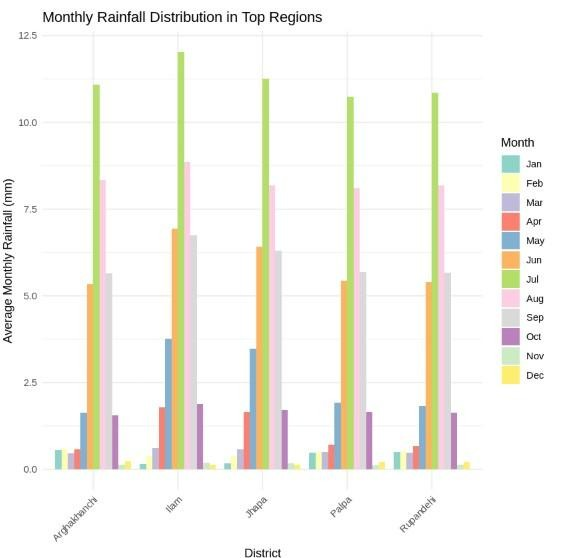
\includegraphics[width=0.5\textwidth]{figures/case2.jpg}
\caption{Figure 8.2: Monthly Rainfall Distribution in Top Rainfall-Prone Districts}
\end{figure}

\subsection*{Conclusion}

This analysis pinpoints both vulnerable districts and high-risk months. Such data-backed insights empower regional authorities to:
\begin{itemize}
    \item Issue timely flood warnings.
    \item Allocate emergency resources.
    \item Plan preventive infrastructure improvements.
\end{itemize}

\section*{Do It Yourself: Scenario-Based Explorations}

In this section, you will apply your R skills to analyze real-world climate scenarios inspired by stories and local observations. Each scenario includes guiding hints and a challenge question to deepen your understanding and decision-making ability using data.

\begin{enumerate}

  \item \textbf{The Warming Winters} \\
  In recent years, winters feel shorter and less cold. Locals say, “We used to need two blankets, now one is enough.” \\
  \textbf{Hints:}
  \begin{itemize}
    \item Check the average winter temperature for each year (e.g., December to February).
    \item Plot the minimum winter temperatures over time.
    \item Compare the current winter averages to those from 10 years ago.
  \end{itemize}
  \textbf{Challenge Question:} \\
  What could happen to winter crops or water storage from snow if this warming trend continues?

  \item \textbf{The Missing Rains} \\
  A farmer says, “It rains all at once or not at all.” The rain hasn’t disappeared—but its pattern seems to have changed. \\
  \textbf{Hints:}
  \begin{itemize}
    \item Calculate how often it rains (number of rainy days) each month.
    \item Plot rainfall amounts by month over the last few years.
    \item Look for months with very heavy rainfall vs. dry periods.
  \end{itemize}
  \textbf{Challenge Question:} \\
  How can farmers plan planting if rainfall becomes less frequent but more intense?

  \item \textbf{Hotspots Emerging} \\
  Heat records are being broken in specific districts while others remain unaffected. Are climate “hotspots” forming? \\
  \textbf{Hints:}
  \begin{itemize}
    \item Calculate average summer temperatures by district.
    \item Identify districts with a steep temperature increase over the last 10 years.
    \item Rank districts by their rate of temperature rise.
  \end{itemize}
  \textbf{Challenge Question:} \\
  Label 3 emerging heat hotspots. What traits (e.g., elevation, urbanization) could explain these areas?

  \item \textbf{Wind Changes in Kathmandu} \\
  Residents have noticed changing wind patterns—some days feel breezier, others still. \\
  \textbf{Hints:}
  \begin{itemize}
    \item Calculate average wind speeds by month over multiple years.
    \item Identify any increasing or decreasing trends.
    \item Highlight the months with the strongest wind activity.
  \end{itemize}
  \textbf{Challenge Question:} \\
  How might wind changes affect air pollution or comfort? Suggest one way Kathmandu could make better use of strong winds.

  \item \textbf{Water Worries in Palpa} \\
  In Palpa, farmers are struggling with reduced and unpredictable rainfall. Water-demanding crops like paddy are suffering. \\
  \textbf{Hints:}
  \begin{itemize}
    \item Identify years in Palpa with low rainfall and high temperatures.
    \item Examine which crops had poor yields in those years.
    \item Compare the performance of rainfed and irrigated crops.
  \end{itemize}
  \textbf{Challenge Question:} \\
  What alternative crops or farming methods would you recommend for Palpa’s farmers during dry conditions? Support your answer using data.

\end{enumerate}
